\documentclass[11pt,a4paper]{article}
\usepackage[utf8]{inputenc}
\usepackage[margin=15mm]{geometry}
\usepackage{tikz}
\usepackage{graphicx}
\usepackage{amsmath}
\usepackage{subfigure}
\usepackage{stix}
\usepackage[font=small,labelfont=bf]{caption}
\graphicspath{{/home/hiago/Documents/Fotos_PFCM/}}
%\usepackage[left=5.2cm,top=2cm,right=1.5cm,bottom=2cm,verbose,nohead,nofoot{geometry}]
\begin{document}
%\maketitle
\includegraphics[scale=0.5]{index}\\
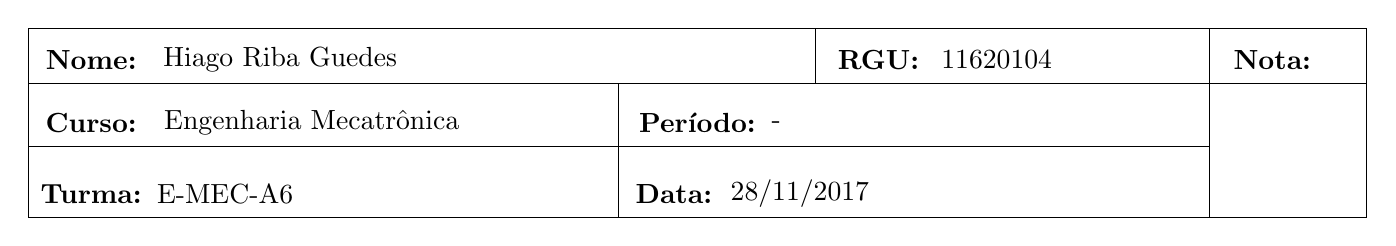
\begin{tikzpicture}
\draw (0,0) rectangle(170mm,24mm);
\draw (0,0) rectangle(170mm,17mm);
\node at(8mm,20mm) {\textbf{Nome: }};
\node at(32mm,20mm) {Hiago Riba Guedes};
\draw(100mm,24mm) rectangle(170mm,17mm);
\draw(150mm,24mm) rectangle(170mm,0mm);
\draw(0,17mm)rectangle(150mm,9mm);
\node at(108mm,20mm){\textbf{RGU: }};
\node at(123mm,20mm){11620104};
\node at(158mm,20mm){\textbf{Nota: }};
\node at(8mm,12mm){\textbf{Curso: }};
\node at(36mm,12mm){Engenharia Mecatrônica};
\node at(8mm,3mm){\textbf{Turma: }};
\node at(25mm,3mm){E-MEC-A6};
\draw (75mm,17mm) rectangle(150mm,0);
\node at(85mm,12mm){\textbf{Período: }};
\node at(95mm,12mm){-};
\node at(82mm,3mm){\textbf{Data: }};
\node at(98mm,3mm){28/11/2017};
%\draw (0,5) rectangle(18,3);
\end{tikzpicture}\\
Professor:Luiz Roberto Miranda \\\\
\begin{tikzpicture}
\draw(0,0)--(80mm,0);
\node at(85mm,0mm){$\medwhitestar$};
\draw(90mm,0)--(170mm,0);
\end{tikzpicture}
\begin{center}
\textbf{Prova Final da disciplina Material de Construção Mecânica}
\end{center}
\textbf{1-Eletricidade (3,0 pts)}\\\\
\underline{Defina:}\\
\textbf{a) Condutividade Elétrica}\\\\
$\sigma=\frac{1}{\rho}$\\\\
É a facilidade do material de conduzir corrente elétrica.É uma propriedade importante para podermos classificarmos os materiais como condutores,semicondutores e isolantes. A fórmula acima quer dizer que a condutividade ($\sigma$) é o inverso da resistividade ($\rho$).
\\\\
\textbf{b) Condução Elétrica e Iônica}\\\\
Nos materiais iônicos é possível haver um movimento resultante de íons carregados, o que produz uma corrente,que é chamada de corrente iônica.\\Corrente Elétrica é o movimento de cargas elétricas na presença de um campo elétrico.\\\\
\textbf{c) Dielétrico, Capacitância e Polarização}\\\\
Um material dielétrico é um isolante elétrico(não metálico) e exibe ou pode ser produzido de modo a exibir uma estrutura de dipolo elétrico de modo a exibir uma estrutura de dipolo elétrico, havendo assim uma separação entre as entidades negativas e positivas eletricamente carregadas.\\\\
\includegraphics{dieletrico}
\\Capacitância está relacionada á quantidade de carga armazenada em cada uma das placas.\\\\
$C=\frac{Q}{V}$\\
Polarização é o processo de alinhamento de um dipolo\\\\
\textbf{d) Semi Condutores}\\\\
Um semicondutor é um material que tem um nível de condutividade entre os extremos de um isolante e de um condutor.\\
Em geral são materiais dopados com uma certa dose de íons de componentes taxados como semicondutores na tabela periódica , como germânio ou silício.\\
Diodo e transistores são exemplos de componentes eletrônicos semicondutivos
\\\\
\textbf{2-Magnetismo (3,0 pts)}\\\\
\textbf{a) Explique a magnetização}\\
\begin{figure}[!htb]
\includegraphics[scale=0.5]{magnetisme_medium}\\
\captionof{figure}{Em 1 temos a ausência de campo magnético.\\
Em 2 temos um campo magnético fraco e um leve aparecimento do alinhamento dos dipolos.\\
Em 3 temos um campo magnético forte e um alinhamento maior dos dipolos em relação ao campo. }
\end{figure}
Depêndencia em relação à suscetibilidade e e à intensidade do campo magnético .\\
Isto é, é o fenômeno que acontece quando os dipolos de um material se alinham de acordo com a direção e a intensidade do campo magnético.
\\\\
\textbf{b) Explique a diferença entre ferromagnetismo,diamagnetismo e paramagnetismo}\\\\
O diamagnetismo é uma forma muito fraca de magnetismo que não é permanente e que persiste apenas enquanto um campo externo está sendo aplicado a ele.Ele é induzido por uma mudança no movimento orbital dos elétrons causada pela aplicação de um campo magnético.E ocorre em direção oposta ao campo aplicado.\\
Paramagnetismo é resultado visto em alguns materiais onde na ausência de campo magnético cada átomo apresenta momentos magnéticos aleatórios .Fazendo com que o material a principio não tenha magnetização resultante. Porém quando se apresenta tal campo,o material apresenta alinhamento com o mesmo.\\
Certos materiais apresentam um momento magnético permanente na ausência de um campo externo,ainda não é compreendido como surgiu tal força ,mas acredita-se que isso seja derivado da estrutura eletrônica do metal.
\\\\
\begin{figure}[!htb]
\includegraphics[scale=1]{lostres}\\
\captionof{figure}{Vetores de polarização dos átomos para cada tipo de material magnético}
\end{figure}
\\\\
\textbf{c) Influência da temperatura: o que é temperatura de Curie?}\\\\
Com o aumento da temperatura, a magnetização de saturação(que é o máximo de magnetização que um material consegue chegar) diminui gradualmente e então cai abruptamente para zero no que é denominada temperatura de Curie.
\\\\
\textbf{d) Explique a diferença entre materiais magnéticos moles e materiais magnéticos duros}\\\\
Um material magnético mole deve apresentar  elevada permeabilidade inicial e baixa coercividade ,ele pode atingir sua magnetização de saturação com a aplicaçaõ de um campo relativamente pequeno (isto é ,é magnetizado e desmagnetizado com facilidade) e ainda possui pequenas perdas de energia por histerese.\\
Um material magnético duro apresenta elevadas remanência, coercividade, e densidade do fluxo de saturação, assim como baixa permeabilidade inicial(são materias mais dificeis de serem magnetizados e de serem desmagnetizados) e grandes perdas de energia por histerese\\
\begin{figure}[!htb]
\includegraphics[scale=0.5]{Untitled}
\captionof{figure}{Onde B é a densidade do fluxo e H a intensidade do campo.}
\end{figure}
\\\\
\textbf{3-Propriedades Opticas (4,0 pts)}\\\\
\textbf{a) O que se entende por Radiação Eletromagnética?}\\\\
A radiação eletromagnética é considerada de natureza ondulatória, consistindo em componentes de campo elétrico e de campo magnético que são perpendiculares entre si e também à direção de propagação.\\\\
\includegraphics[]{onda.jpg}
\\\\
\textbf{b) O que é o LED("light-emitting diode")}\\\\
É um componente semicondutor que consegue transformar energia elétrica em energia luminosa.
\\\\
\textbf{c) Quais são os principais tipos de laser?}\\\\
Laser de estado sólido,laser de gás ionizado,laser á gás,de vapor metálico,laser líquido,laser semicondutor.
\\\\
\textbf{d) O que são as fibras ópticas?}\\\\
São filamentos flexíveis e transparentes que possuem a propriedade de transmitir fótons/luz .O que melhora a velocidade de transimissão e reduz a taxa de erros da dita trasmissão eletrônica.São materiais que não sofrem interferência magnética.
\\\\
\end{document}